\documentclass[aspectratio=169,10pt]{beamer}

\usetheme{Madrid}
\usecolortheme{default}
\setbeamertemplate{navigation symbols}{}
\setbeamertemplate{footline}{}
\usepackage{amsmath,amssymb,booktabs,array}
\usepackage{graphicx}
\usepackage{tikz}
\usetikzlibrary{arrows.meta,positioning,calc,fit,shapes.geometric}
\usepackage{fontspec}
\usepackage{unicode-math}
\usepackage{ucharclasses}

\setmainfont{Droid Sans Fallback}
\setsansfont{Droid Sans Fallback}
\setmonofont{Droid Sans Fallback}
\setmathfont{Latin Modern Math}
\newfontfamily\latinfont{DejaVu Sans}
\setTransitionsForLatin{\latinfont}{\normalfont}

\newcommand{\en}[1]{{\latinfont #1}}
\newcommand{\mt}[1]{\text{\en{#1}}}
\newcommand{\mop}[1]{\mathop{\text{\en{#1}}}}
\newcommand{\dive}{\en{DRIP}}
\newcommand{\arc}{\en{ARC}}
\newcommand{\lru}{\en{LRU}}
\newcommand{\fifo}{\en{FIFO}}
\newcommand{\ond}{\en{OnDemand}}
\newcommand{\gptc}{\en{GPTCache}}

\title[\dive]{\dive{}: \en{Drift-aware Insertion with Visibility-aware Evidence}}
\subtitle{\en{Shared Hot-Tier Management for Multi-Agent RAG}}
\author{}
\date{\en{2026-06-22}}

\begin{document}

\begin{frame}
  \titlepage
\end{frame}

\begin{frame}{Problem: Shared RAG Hot Cache}
  \begin{columns}[T]
    \begin{column}{0.48\textwidth}
      \begin{block}{Setting}
        \[
          C_t \subset \mathcal{D}, \qquad |C_t| \le B
        \]
        \small
        A small persistent hot tier is shared by multiple agents/users.
      \end{block}
    \end{column}
    \begin{column}{0.48\textwidth}
      \begin{block}{Goal}
        \small
        Keep evidence that will answer future windows while limiting cold fetches
        and rewrite cost.
      \end{block}
    \end{column}
  \end{columns}

  \vspace{0.6em}
  \begin{alertblock}{Core cache-management question}
    Which documents should be inserted and retained when user demand shifts
    and useful evidence may be hidden behind multi-hop reasoning?
  \end{alertblock}
\end{frame}

\begin{frame}{Motivation I: Demand Drift}
  \begin{columns}[T]
    \begin{column}{0.61\textwidth}
      \centering
      
\includegraphics[width=\linewidth,height=0.70\textheight,keepaspectratio]{/home/jyliu/RAG-project/motivation/paper_figs/intro/fig0_intro_user_query_topic_drift.pdf}
    \end{column}
    \begin{column}{0.35\textwidth}
      \small
      \begin{block}{Observation}
        Agent/user requests are non-stationary.
      \end{block}
      \begin{block}{Cache failure}
        Access-history policies keep yesterday's working set.
      \end{block}
      \begin{alertblock}{Need}
        A controller for \textbf{when} and \textbf{how much} the hot tier should move.
      \end{alertblock}
    \end{column}
  \end{columns}

\end{frame}

\begin{frame}{Motivation II: Evidence Visibility}
  \centering
  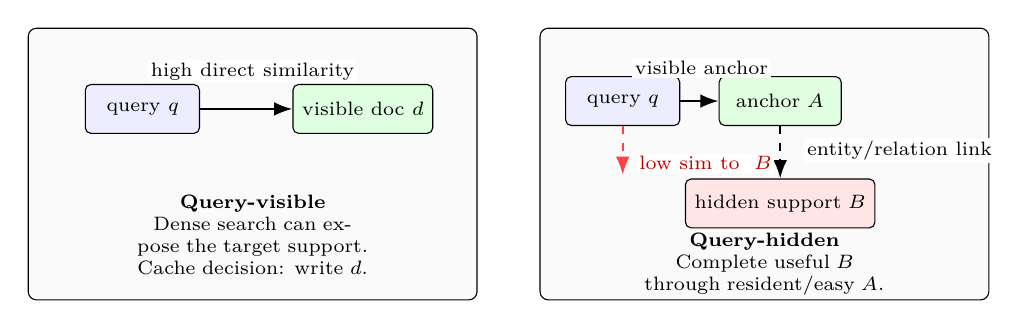
\begin{tikzpicture}[
    font=\scriptsize,
    >=Latex,
    panel/.style={draw, rounded corners=3pt, fill=gray!4, minimum width=5.7cm, minimum height=3.45cm},
    box/.style={draw, rounded corners=2pt, minimum width=1.45cm, minimum height=0.62cm, align=center, fill=blue!7},
    good/.style={draw, rounded corners=2pt, minimum width=1.55cm, minimum height=0.62cm, align=center, fill=green!12},
    hid/.style={draw, rounded corners=2pt, minimum width=1.65cm, minimum height=0.62cm, align=center, fill=red!10},
    lab/.style={fill=white, inner sep=1pt}
  ]
    \node[panel] at (-3.25,0.55) {};
    \node[panel] at (3.25,0.55) {};

    \node[box] (q1) at (-4.65,1.25) {query $q$};
    \node[good] (d) at (-1.85,1.25) {visible doc $d$};
    \node[lab] at (-3.25,1.72) {\en{high direct similarity}};
    \draw[->,thick] (q1) -- (d);
    \node[align=center,text width=4.7cm] at (-3.25,-0.35)
      {\textbf{Query-visible}\\Dense search can expose the target support.\\Cache decision: write $d$.};

    \node[box] (q2) at (1.45,1.35) {query $q$};
    \node[good] (a) at (3.45,1.35) {anchor $A$};
    \node[hid] (b) at (3.45,0.05) {hidden support $B$};
    \node[lab] at (2.45,1.77) {\en{visible anchor}};
    \draw[->,thick] (q2) -- (a);
    \draw[->,thick,dashed] (a) -- (b);
    \node[lab,anchor=west] at (3.75,0.72) {\en{entity/relation link}};
    \draw[->,red!75,thick,dashed] (q2.south) -- ++(0,-0.62);
    \node[fill=white,inner sep=1pt,text=red!75!black,anchor=west] at (1.62,0.56)
      {\en{low sim to } $B$};
    \node[align=center,text width=4.8cm] at (3.25,-0.72)
      {\textbf{Query-hidden}\\Complete useful $B$ through resident/easy $A$.};
  \end{tikzpicture}

  \vspace{0.3em}
  \begin{alertblock}{Need}
    A cache policy for \textbf{what} evidence to move: direct support and hidden support units.
  \end{alertblock}
\end{frame}

\begin{frame}{Positioning}
  \scriptsize
  \begin{table}
  \centering
  \setlength{\tabcolsep}{3pt}
  \begin{tabular}{p{0.32\textwidth}ccc}
    \toprule
    Method family & Explicit drift signal? & Uses semantics? & Completes hidden support? \\
    \midrule
    \lru{}/\fifo{}/\en{TinyLFU} & no & no & no \\
    \gptc{}/semantic cache & no & query-answer & no \\
    \arc{} / Agent RAG Cache & no & limited & no \\
    \en{GraphRAG}/\en{HippoRAG}/online fetch & no & yes & not persistent \\
    \dive{} & prototype & evidence-level & yes \\
    \bottomrule
  \end{tabular}
  \end{table}

  \begin{alertblock}{\dive{}'s object}
    Persistent document hot-tier management with an explicit drift signal,
    not one-shot retrieval or passive recency adaptation.
  \end{alertblock}
\end{frame}

\begin{frame}{\dive{} System Diagram}
  \centering
  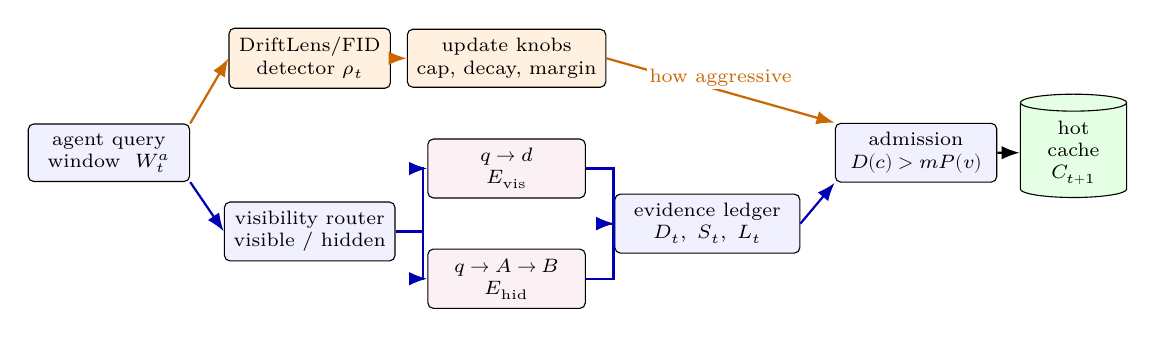
\begin{tikzpicture}[
    font=\scriptsize,
    >=Latex,
    proc/.style={draw, rounded corners=2pt, align=center, minimum width=2.05cm, minimum height=0.70cm, fill=blue!6},
    branch/.style={draw, rounded corners=2pt, align=center, minimum width=2.0cm, minimum height=0.64cm, fill=purple!6},
    note/.style={draw, rounded corners=2pt, align=center, minimum width=2.05cm, minimum height=0.64cm, fill=orange!12},
    cache/.style={draw, cylinder, shape border rotate=90, aspect=0.24, align=center, minimum height=1.0cm, minimum width=1.35cm, fill=green!10},
    lab/.style={fill=white, inner sep=1pt}
  ]
    \node[proc] (q) at (-5.6,0.25) {\en{agent query}\\\en{window } $W_t^a$};
    \node[note] (drift) at (-3.05,1.45) {\en{DriftLens/FID}\\\en{detector }$\rho_t$};
    \node[note] (knobs) at (-0.55,1.45) {\en{update knobs}\\\en{cap, decay, margin}};
    \node[proc] (router) at (-3.05,-0.75) {\en{visibility router}\\\en{visible / hidden}};
    \node[branch] (vis) at (-0.55,0.05) {$q\rightarrow d$\\$E_{\mt{vis}}$};
    \node[branch] (hid) at (-0.55,-1.35) {$q\rightarrow A\rightarrow B$\\$E_{\mt{hid}}$};
    \node[proc, minimum width=2.35cm] (ledger) at (2.0,-0.65) {\en{evidence ledger}\\$D_t,\ S_t,\ L_t$};
    \node[proc] (admit) at (4.65,0.25) {\en{admission}\\$D(c)>mP(v)$};
    \node[cache] (cache) at (6.65,0.25) {\en{hot}\\\en{cache}\\$C_{t+1}$};

    \draw[->,thick,orange!80!black] (q.north east) -- (drift.west);
    \draw[->,thick,orange!80!black] (drift) -- (knobs);
    \draw[->,thick,orange!80!black] (knobs.east) -- node[lab,above]{\en{how aggressive}} (admit.north west);

    \draw[->,thick,blue!70!black] (q.south east) -- (router.west);
    \draw[->,thick,blue!70!black] (router.east) -- ++(0.35,0) |- (vis.west);
    \draw[->,thick,blue!70!black] (router.east) -- ++(0.35,0) |- (hid.west);
    \draw[->,thick,blue!70!black] (vis.east) -- ++(0.35,0) |- (ledger.west);
    \draw[->,thick,blue!70!black] (hid.east) -- ++(0.35,0) |- (ledger.west);
    \draw[->,thick,blue!70!black] (ledger.east) -- (admit.south west);
    \draw[->,thick] (admit) -- (cache);
  \end{tikzpicture}

  \vspace{0.5em}
  \begin{block}{Separation}
    $\rho_t$ controls \textbf{when/how aggressively} to update;
    evidence scores decide \textbf{which documents} to insert.
  \end{block}
\end{frame}

\begin{frame}{Evidence Scores}
  \small
  \begin{columns}[T]
    \begin{column}{0.47\textwidth}
      \begin{block}{Query-visible}
        \[
          E_{\mt{vis}}(q,d)
          =
          \mop{max}(0,\mop{sim}(q,d))\cdot r(d)
        \]
        \centering
        \en{direct query neighborhood}
      \end{block}
    \end{column}
    \begin{column}{0.49\textwidth}
      \begin{block}{Query-hidden}
        \[
          E_{\mt{hid}}(q,B|A)
          =
          \mop{sim}(\phi(q,A),B)\cdot \mop{link}(A,B)\cdot \mop{cue}(q,B)
        \]
        \centering
        \en{complete hidden support through anchor}
      \end{block}
    \end{column}
  \end{columns}

  \begin{block}{Unified ledger}
    \[
      D_t(d)=D_{\mt{vis},t}(d)+D_{\mt{hid},t}(d)+\lambda_{\mt{unit}}L_t(d),
      \qquad
      P_t(d)=S_t(d)+D_t(d).
    \]
  \end{block}
\end{frame}

\begin{frame}{Algorithm: \dive{} Cache Maintenance}
  \small
  \begin{block}{Input / Output}
    $W_t,\ C_t,\ \mathcal{D}\quad \longrightarrow \quad C_{t+1},\ |C_{t+1}|\le B$
  \end{block}

  \begin{table}
  \centering
  \renewcommand{\arraystretch}{1.18}
  \setlength{\tabcolsep}{7pt}
  \begin{tabular}{rl}
    \toprule
    1 & $S_t \leftarrow \mop{serve}(W_t,C_t)$ \\
    2 & $\rho_t \leftarrow \mop{drift}(W_t,C_t)$ \\
    3 & $E_t \leftarrow E_{\mt{vis}}(q,d)\ \cup\ E_{\mt{hid}}(q,B|A)$ \\
    4 & $D_t \leftarrow \lambda D_{t-1}+E_t,\qquad P_t \leftarrow S_t+D_t$ \\
    5 & $C_{t+1}\leftarrow \mop{admit}(C_t,D_t,P_t,\rho_t)$ \\
    \bottomrule
  \end{tabular}
  \end{table}

  \begin{alertblock}{Key difference}
    \dive{} chooses both \textbf{when to move} and \textbf{which evidence to move}:
    visible $q\rightarrow d$ and hidden $q\rightarrow A\rightarrow B$.
  \end{alertblock}
\end{frame}

\begin{frame}{Admission Rule}
  \centering
  \[
    \mop{admit}(c,v)
    \Longleftrightarrow
    D_t(c)>m_t P_t(v)
  \]

  \vspace{0.5em}
  \begin{columns}[T]
    \begin{column}{0.31\textwidth}
      \begin{block}{Direct first}
        \small
        Do not evict current visible evidence for speculative bridges.
      \end{block}
    \end{column}
    \begin{column}{0.31\textwidth}
      \begin{block}{Support-unit lease}
        \small
        If $B$ is inserted, its contributing anchors $A_i$ receive decayed credit.
      \end{block}
    \end{column}
    \begin{column}{0.31\textwidth}
      \begin{block}{Simple priority}
        \small
        No public redundancy/hubness term:
        resident priority remains $S+D$.
      \end{block}
    \end{column}
  \end{columns}

  \vspace{0.35em}
  \begin{alertblock}{Update cost is controlled, not directly subtracted}
    No extra write-penalty term is added to $P_t(d)$ or $D_t(c)$.
    Update cost is controlled by per-window budget, duplicate filtering,
    and the margin gate above, then reported as a cost metric.
  \end{alertblock}
\end{frame}

\begin{frame}{Benchmark Suite}
  \scriptsize
  \begin{table}
  \centering
  \setlength{\tabcolsep}{2.4pt}
  \begin{tabular}{
    >{\raggedright\arraybackslash}p{0.16\textwidth}
    >{\raggedright\arraybackslash}p{0.22\textwidth}
    >{\raggedright\arraybackslash}p{0.52\textwidth}}
    \toprule
    Branch & Dataset & Claim tested \\
    \midrule
    \en{Query-visible} &
    \en{2Wiki comparison} &
    Post-drift cache-only answerability and recall. \\
    \en{Query-hidden} &
    \en{2Wiki bridge-comparison}, \en{MuSiQue} &
    Complete and retain hidden support units $A+B$. \\
    \en{Combined diagnostic} &
    \en{2Wiki topic-shift bridge} &
    Stress test for drift plus hidden support scheduling. \\
    \bottomrule
  \end{tabular}
  \end{table}

  \begin{block}{Unified main baseline suite}
    \lru{} / \fifo{} / \gptc{} / \arc{} /
    \dive{}-\en{Dense} \en{(w/o hidden)} / \dive{} / \ond{}.
    \en{For query-visible data, } \dive{} \en{ uses the dense/direct route;
    hidden branch additionally reports } \dive{}-\en{ESC}.
  \end{block}

  \begin{alertblock}{Metric split}
    All result tables use four metrics only:
    \en{Has-Answer Rate}, normalized \en{AMAT}, \en{Recall@5}, and update cost.
  \end{alertblock}
\end{frame}

\begin{frame}{Metrics: ARC-Compatible Names}
  \small
  \begin{table}
  \centering
  \setlength{\tabcolsep}{7pt}
  \begin{tabular}{lp{0.58\textwidth}}
    \toprule
    Metric & Meaning \\
    \midrule
    \en{Has-Answer Rate}$\uparrow$ &
    Fraction of queries whose required support is already answerable from the hot cache. \\
    \en{AMAT}$\downarrow$ &
    Normalized average memory access time; we count cold support misses and add serve-time full-index fetch overhead for \ond{}. \\
    \en{Recall@5}$\uparrow$ &
    Top-5 retrieval quality from the effective cache. \\
    \en{Update Cost}$\downarrow$ &
    Number of cache writes/evictions. Lower is better when quality is comparable. \\
    \bottomrule
  \end{tabular}
  \end{table}

  \vspace{0.4em}
  \begin{alertblock}{Reading rule}
    Hidden-support and reuse numbers are diagnostic only; they are not shown in
    main result tables.
  \end{alertblock}
\end{frame}

\begin{frame}{Query-Visible Branch: 2Wiki Comparison}
  \scriptsize
  \en{2Wiki comparison, full-gradual query shift; pool=31,907, KB=6,250; 100 windows x 50 queries}

  \begin{table}
  \centering
  \renewcommand{\arraystretch}{1.08}
  \setlength{\tabcolsep}{5.5pt}
  \begin{tabular}{lrrrr}
    \toprule
    Method & \shortstack{\en{Has-Answer}\\\en{Rate}$\uparrow$} & \en{AMAT}$\downarrow$ & \en{Recall@5}$\uparrow$ & \shortstack{\en{Update}\\\en{Cost}$\downarrow$} \\
    \midrule
    \lru{} & 25.9 & 1.09 & 34.8 & 1835 \\
    \gptc{} & 23.6 & 1.25 & 22.2 & 6375 \\
    \arc{} & 19.5 & 1.22 & 34.5 & 9248 \\
    \dive{} & \textbf{32.0} & \textbf{1.07} & \textbf{40.4} & 7657 \\
    \ond{}$^*$ & 28.7 & 31.33 & 95.8 & \textbf{0} \\
    \bottomrule
  \end{tabular}
  \end{table}

  \begin{block}{Reading}
    \dive{} is the best persistent cache-only writer on answerability,
    normalized \en{AMAT}, and post-shift \en{Recall@5}. $^*$\ond{} includes
    serve-time full-index delay in \en{AMAT}.
  \end{block}
\end{frame}

\begin{frame}{Hidden Multi-Hop Construction}
  \centering
  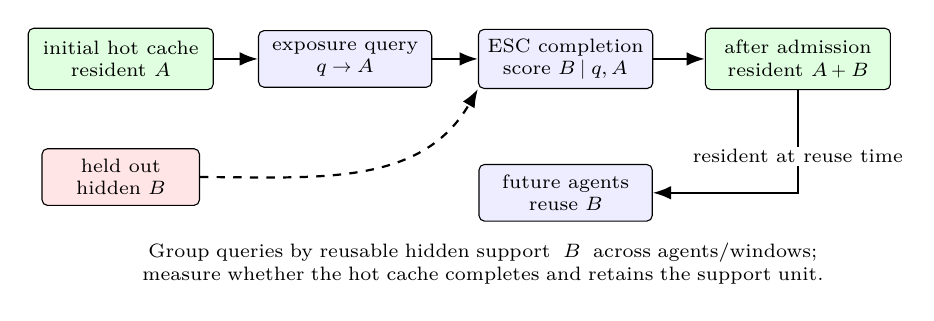
\begin{tikzpicture}[
    font=\scriptsize,
    >=Latex,
    flow/.style={draw, rounded corners=2pt, align=center, minimum width=2.2cm, minimum height=0.72cm, fill=blue!7},
    cache/.style={draw, rounded corners=2pt, align=center, minimum width=2.35cm, minimum height=0.78cm, fill=green!12},
    hold/.style={draw, rounded corners=2pt, align=center, minimum width=2.0cm, minimum height=0.72cm, fill=red!10},
    lab/.style={fill=white, inner sep=1pt}
  ]
    \node[cache] (init) at (-4.6,0.85) {\en{initial hot cache}\\resident $A$};
    \node[hold] (held) at (-4.6,-0.65) {\en{held out}\\hidden $B$};
    \node[flow] (q) at (-1.75,0.85) {\en{exposure query}\\$q\rightarrow A$};
    \node[flow] (esc) at (1.05,0.85) {\en{ESC completion}\\score $B\mid q,A$};
    \node[cache] (after) at (4.0,0.85) {\en{after admission}\\resident $A+B$};
    \node[flow] (reuse) at (1.05,-0.85) {\en{future agents}\\reuse $B$};

    \draw[->,thick] (init) -- (q);
    \draw[->,thick] (q) -- (esc);
    \draw[->,thick,dashed] (held.east) to[out=0,in=-120] (esc.south west);
    \draw[->,thick] (esc) -- (after);
    \draw[->,thick] (after.south) |- node[lab,below,pos=0.27]{\en{resident at reuse time}} (reuse.east);

    \node[align=center,text width=8.8cm] at (0,-1.75)
      {\en{Group queries by reusable hidden support } $B$ \en{ across agents/windows; measure whether the hot cache completes and retains the support unit.}};
  \end{tikzpicture}

  \vspace{0.5em}
  \begin{alertblock}{Clean main setting}
    No topic shift: first prove hidden multi-hop cache management itself.
  \end{alertblock}
\end{frame}

\begin{frame}{Query-Hidden Branch: 2Wiki and MuSiQue}
  \scriptsize
  \en{Hidden support reuse without topic shift; KB=750; 20 windows x 25 queries}

  \begin{table}
  \centering
  \renewcommand{\arraystretch}{1.08}
  \setlength{\tabcolsep}{4.2pt}
  \begin{tabular}{llrrrr}
    \toprule
    Dataset & Method & \shortstack{\en{Has-Answer}\\\en{Rate}$\uparrow$} & \en{AMAT}$\downarrow$ & \en{Recall@5}$\uparrow$ & \shortstack{\en{Update}\\\en{Cost}$\downarrow$} \\
    \midrule
    \en{2Wiki} & \lru{} & \textbf{11.6} & \textbf{1.71} & \textbf{30.6} & \textbf{108} \\
    \en{2Wiki} & \arc{} & 0.2 & 2.89 & 15.5 & 1442 \\
    \en{2Wiki} & \dive{} & 3.6 & 2.17 & 21.1 & 824 \\
    \en{2Wiki} & \ond{}$^*$ & 11.8 & 20.26 & 48.8 & 0 \\
    \midrule
    \en{MuSiQue} & \lru{} & \textbf{10.8} & \textbf{1.36} & \textbf{38.0} & \textbf{100} \\
    \en{MuSiQue} & \arc{} & 2.4 & 2.08 & 20.3 & 1796 \\
    \en{MuSiQue} & \dive{} & 7.2 & 1.69 & 26.5 & 800 \\
    \en{MuSiQue} & \ond{}$^*$ & 8.8 & 21.64 & 40.0 & 0 \\
    \bottomrule
  \end{tabular}
  \end{table}

  \begin{block}{Reading}
    \dive{} clearly improves over \arc{} on hidden multi-hop admission, but
    pure temporal locality remains a strong cache-only baseline in this stream.
    $^*$\ond{} gets high recall by paying serve-time full-index delay.
  \end{block}
\end{frame}

\begin{frame}{Current Limitation: Drift + Hidden Support}
  \scriptsize
  \en{2Wiki topic-shift bridge reuse, pool=22,984, KB=750, 100 windows x 50 queries; unified baselines}

  \begin{table}
  \centering
  \renewcommand{\arraystretch}{1.08}
  \setlength{\tabcolsep}{5.0pt}
  \begin{tabular}{lrrrr}
    \toprule
    Method & \shortstack{\en{Has-Answer}\\\en{Rate}$\uparrow$} & \en{AMAT}$\downarrow$ & \en{Recall@5}$\uparrow$ & \shortstack{\en{Update}\\\en{Cost}$\downarrow$} \\
    \midrule
    \lru{} & 0.2 & 3.70 & 6.1 & 3768 \\
    \arc{} & 0.0 & \textbf{3.64} & 2.4 & \textbf{2785} \\
    \dive{} & \textbf{0.4} & 3.67 & 4.2 & 4247 \\
    \ond{}$^*$ & 1.3 & 44.96 & 48.2 & 0 \\
    \bottomrule
  \end{tabular}
  \end{table}

  \begin{alertblock}{Honest status}
    Under simultaneous topic drift and hidden support, persistent-cache methods
    remain weak; $^*$\ond{} is strong only by paying serve-time full-index delay.
    The detector/scheduler is the open component.
  \end{alertblock}
\end{frame}

\begin{frame}{Real Agent Trace Diagnostic: Mind2Web}
  \scriptsize
  \begin{columns}[T]
    \begin{column}{0.50\textwidth}
      \begin{block}{Construction}
        \begin{itemize}
          \setlength\itemsep{0.25em}
          \item Raw data: human web-agent trajectories on real websites.
          \item Document $d$: a normalized website element or control.
          \item Query $q_t$: task text, website/domain, and previous actions.
          \item Support unit: previous target element $A$ plus next target element $B$.
          \item Grouping: collect tasks with the same future target $B$ across agents.
          \item Initialization: keep some historical anchors and hold out reusable targets.
        \end{itemize}
      \end{block}
    \end{column}

    \begin{column}{0.47\textwidth}
      \begin{block}{First-pass result: KB=500, 20x25}
        \centering
        \scriptsize
        \renewcommand{\arraystretch}{1.06}
        \setlength{\tabcolsep}{2.0pt}
        \begin{tabular}{lrrrr}
          \toprule
          Method & \shortstack{\en{Has-Answer}\\\en{Rate}} & \en{AMAT} & \en{Recall@5} & \shortstack{\en{Update}\\\en{Cost}} \\
          \midrule
          \lru{} & 48.8 & 0.57 & 48.0 & \textbf{41} \\
          \en{AgentRAG} & 50.8 & 0.60 & 47.2 & 1009 \\
          \dive{}-\en{Dense} & \textbf{59.8} & \textbf{0.51} & 47.8 & 395 \\
          \dive{}-\en{Hidden} & 52.6 & 0.62 & \textbf{48.6} & 258 \\
          \bottomrule
        \end{tabular}
      \end{block}
      \begin{alertblock}{Reading}
        Mind2Web is a real-agent shared-cache diagnostic. Against the hubness-aware
        \en{AgentRAG} baseline, \dive{}-\en{Dense} gives the best answerability
        and \en{AMAT}; \dive{}-\en{Hidden} gives the best \en{Recall@5} with low writes.
      \end{alertblock}
    \end{column}
  \end{columns}
\end{frame}

\begin{frame}{Contributions}
  \small
  \begin{enumerate}
    \item \textbf{Problem}: shared RAG hot-cache management under demand drift
      and evidence visibility shift.
    \item \textbf{Method}: separate drift control from visibility-aware evidence admission.
    \item \textbf{Mechanism}: hidden support completion and support-unit lease.
    \item \textbf{Evidence}: query-visible 2Wiki comparison improves over cache-only
      baselines; query-hidden 2Wiki/MuSiQue improves support residency over ARC.
    \item \textbf{Open problem}: robust budget scheduling when topic drift and
      hidden multi-hop evidence happen together.
  \end{enumerate}
\end{frame}

\begin{frame}{Experimental Caveats and Next Steps}
  \scriptsize
  \begin{columns}[T]
    \begin{column}{0.49\textwidth}
      \begin{block}{What is solid}
        \begin{itemize}
          \setlength\itemsep{0.25em}
          \item Query-visible/direct branch is the most stable result:
          semantic demand plus serve utility improves persistent cache quality
          under drift.
          \item Hidden branch shows signal over \arc{}-style admission on
          hidden target reuse and write efficiency.
          \item Mind2Web confirms that shared hot-cache reuse appears in real
          web-agent traces.
        \end{itemize}
      \end{block}
    \end{column}

    \begin{column}{0.49\textwidth}
      \begin{alertblock}{What is not solved yet}
        \begin{itemize}
          \setlength\itemsep{0.25em}
          \item Strong temporal locality makes \lru{}/\fifo{} surprisingly hard
          baselines in hidden-reuse benchmarks.
          \item Graph/PPR propagation is noisy on real entity graphs because hub
          entities mix true bridge pages with many distractors.
          \item Hidden support still needs better $A+B$ pair retention:
          writing $B$ alone does not guarantee answerability.
          \item Current drift detector is preliminary; simultaneous drift +
          hidden support needs better budget scheduling.
          \item Mind2Web is a real-agent diagnostic, but closer to repeated UI
          target reuse than Wikipedia-style hidden bridge reasoning.
        \end{itemize}
      \end{alertblock}
    \end{column}
  \end{columns}

  \begin{block}{Next step}
    Strengthen relation/entity linking and pair retention, then re-evaluate
    hidden support under stricter streams where recency-only policies cannot
    win from initialization and temporal locality alone.
  \end{block}
\end{frame}

\begin{frame}{Takeaway}
  \centering
  \Large
  \[
    \text{\en{Demand drift: when to move}}
  \]
  \[
    \text{\en{Evidence visibility: what to move}}
  \]

  \vspace{0.5em}
  \begin{alertblock}{\dive{}}
    A shared RAG hot-cache manager that keeps both
    $q\rightarrow d$ visible evidence and $q\rightarrow A\rightarrow B$
    hidden support units.
  \end{alertblock}
\end{frame}

\end{document}
